\section{FIREbox: a novel cosmological simulation}
Scale and resolution are important for simulations. Astrophysicists must balance large volume and high detail, both of which cost computing power. The large volume simulations allow us to closely study intergalactic systems and to collect large amounts of statistical information about galaxies \citep{feldmannFIREboxSimulatingGalaxies2022}. However, a higher resolution "zoom in" simulation such as FIRE in the Field \citep{fittsFireFieldSimulating2017} allows us to better simulate the internal physics of the galaxies themselves.

This paper will examine data from FIREbox \citep{feldmannFIREboxSimulatingGalaxies2022}. This cosmological simulation does not have the largest volume, nor is it the most detailed. Rather, it incorporates a balance of high detail and large scale (see Figure \ref{fig:feldmann-dynrange}), which together give it the highest dynamical range of any cosmological simulation to this date.

\begin{figure}
    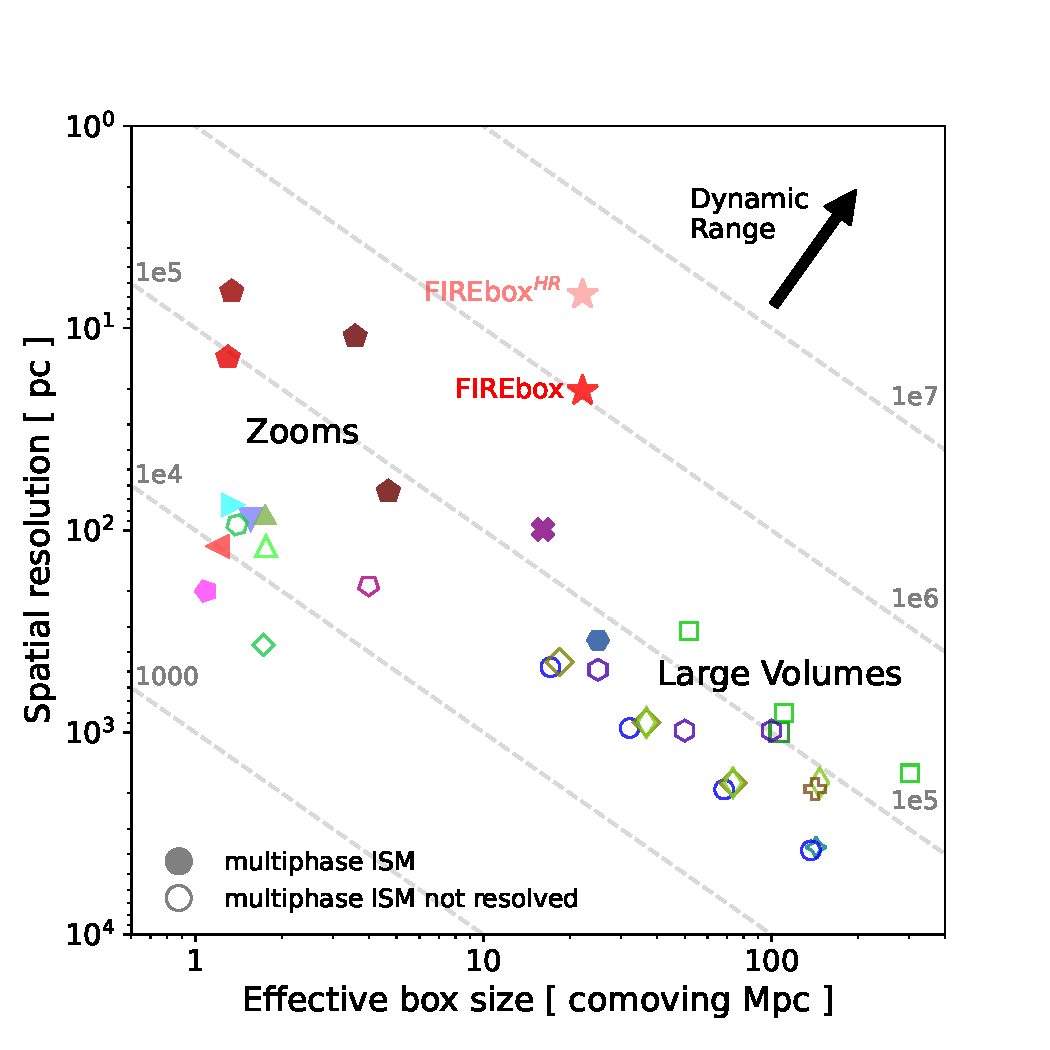
\includegraphics[width=\textwidth/2]{figs/feldmann/fig2a}
    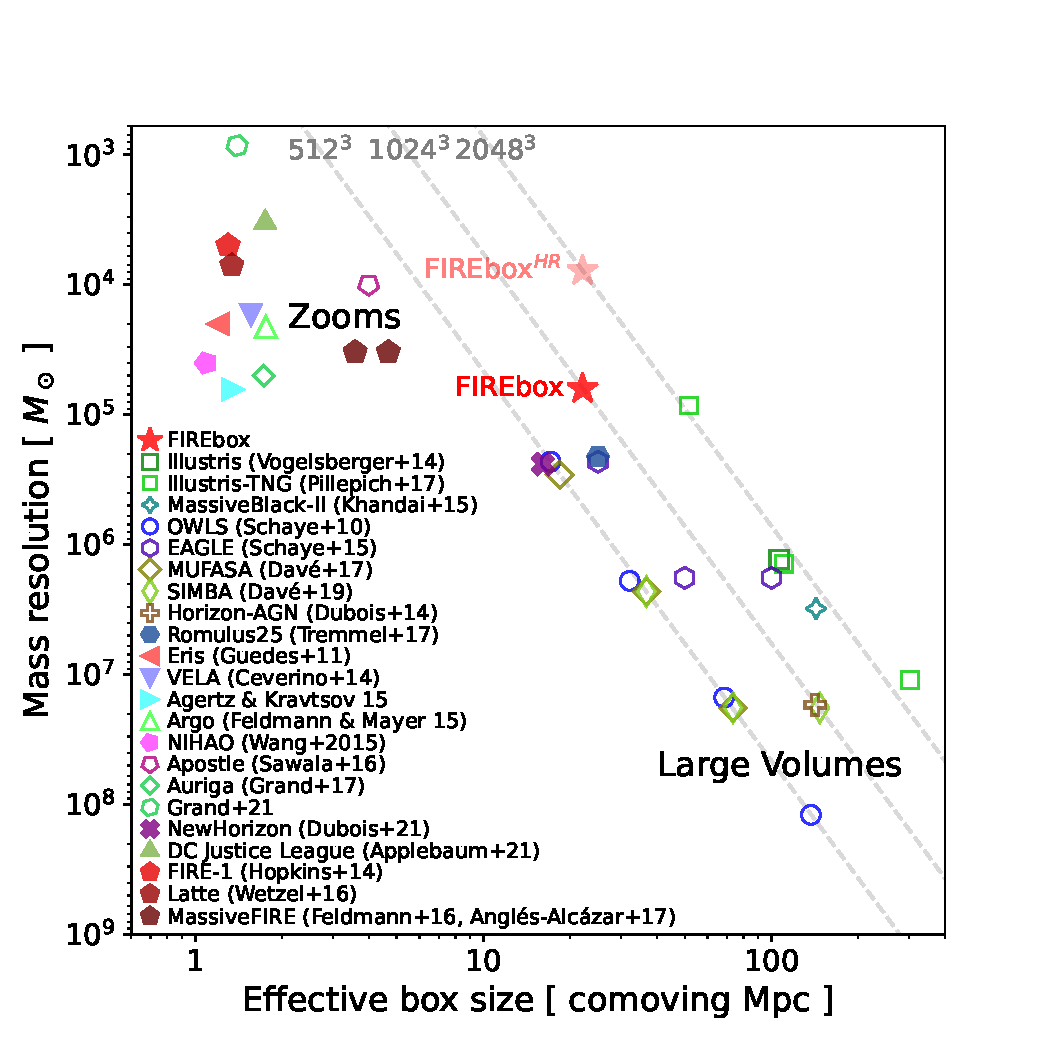
\includegraphics[width=\textwidth/2]{figs/feldmann/fig2b}
    
    \caption{A comparison the size and detail of cosmological simulations. There is a tradeoff between scale and resolution, where a total increase in both means a higher dynamic range at the cost of computer performance. FIREbox has the highest dynamic range, and therefore the highest computational cost.}

    \label{fig:feldmann-dynrange}
\end{figure}

\section{The data}
Over the course of the evolution of the FIREbox simulation, 1201 snapshots describing the state of the universe were collected \citep{feldmannFIREboxSimulatingGalaxies2022}. They were approximately evenly spaced out in time and included the positions of the particles, their densities, metallicities, star-formation rates, and other properties. The particle data was reduced by grouping the particles into their respective galaxies and dark matter halos. The authors used the AMIGA Halo Finder \citep[AHF;][]{knollmannAhfAMIGAHALO2009} to sort the halos into two hierarchical categories: main halos and sub-halos. This, in turn, allowed them to categorize the galaxies by hosts and satellites, respectively. The reduced data, known as the galaxy and halo catalog, includes galaxy information such as position, radius, mass and star formation rate, as well as data about the dark matter halos around those galaxies. I will be mostly using snapshot 1201, the final state of the simulation. This snapshot depicts the simulated present day.

Each parameter for the galaxies is split between a few different definitions. For the purpose of this thesis, I will use the following definitions unless otherwise specified. The galaxy's radius $R_{50}$ is defined to be the radius containing 50\% of its stellar mass, as determined by AHF. The galaxy's mass $M_\star$ is defined to be the mass of the stars contained within $R_{50}$. I will not include dark matter in this definition. The reader should note that this is not the only way to define these parameters. Due to the fluid nature of matter on a galactic scale, it is often arbitrary as to whether a given particle belongs to a given galaxy. Alternate definitions include different thresholds for the radius, such as $R_{80}$, and different kinds of matter included in the mass, such as gas matter and dark matter.

Other parameters that I will use are a galaxy's position in space and its flyby distance---a satellite galaxy's minimum distance to its host galaxy. All distances (including radius) are measured in terms of the co-moving parameter $h$, a time-dependent scaling factor of the universe. In the final state of FIREbox, $h = 0.6774 \text{ kpc}$. 

\cite{mcconnachieOBSERVEDPROPERTIESDWARF2012} compiled a number of data sets for low-mass galaxies in the Local Group. One data set includes the galaxies' radii and another contains their masses. The radius is defined slightly differently in this case. It is the half-light radius, the radius from which half of the galaxy's light is emitted.
Klein et al. (in prep) shows that the half-light radius is functionally identical to $R_{50}$. $M_\star$ is calculated by assuming a mass-light ratio of one, meaning that the brightness per unit mass is equal to the Sun.

To get this data in a usable form, I first dumped the text-based datasets into pandas spreadsheets and removed rows with missing data. I then merged the datasets by galaxy name. For galaxies whose names were reported differently on the different sheets, I merged them by hand. I then cast the mass and radius to float64 for use in the analysis.

% TODO: discuss figs 2.1 and 2.2 earlier

\begin{figure}
    \includegraphics*[width=\textwidth]{figs/feldmann/fig1.pdf}
    \label{fig:feldmann-visual}
    \caption{
        From: \cite{feldmannFIREboxSimulatingGalaxies2022}. A representation of the FIREbox simulation. The first two rows depict the state of the simulation at three different time points; the rightmost images depict the simulation in the present time. The top row depicts dark matter in blue and stellar matter in white, while the middle row depicts gas. The bottom row shows a galaxy at different scales. As one can see, matter collects into galaxies and systems of galaxies over the course of the simulated universe's evolution. These galaxies take on a variety of sizes, and they share threads of gas and are contained within hierarchical halos of dark matter.
    }
\end{figure}

\begin{figure}
    \centering
    \includegraphics*[width=\textwidth*11/10]{figs/me/locations.pdf}
    \caption*{
        A 2D visualization of FIREbox; the X and Y coordinates of each galaxy. Host galaxies are depicted as gray circles, and satellites galaxies are triangles that are colored by the distance to their host galaxy. 
    }
\end{figure}

\begin{figure}
    \centering
    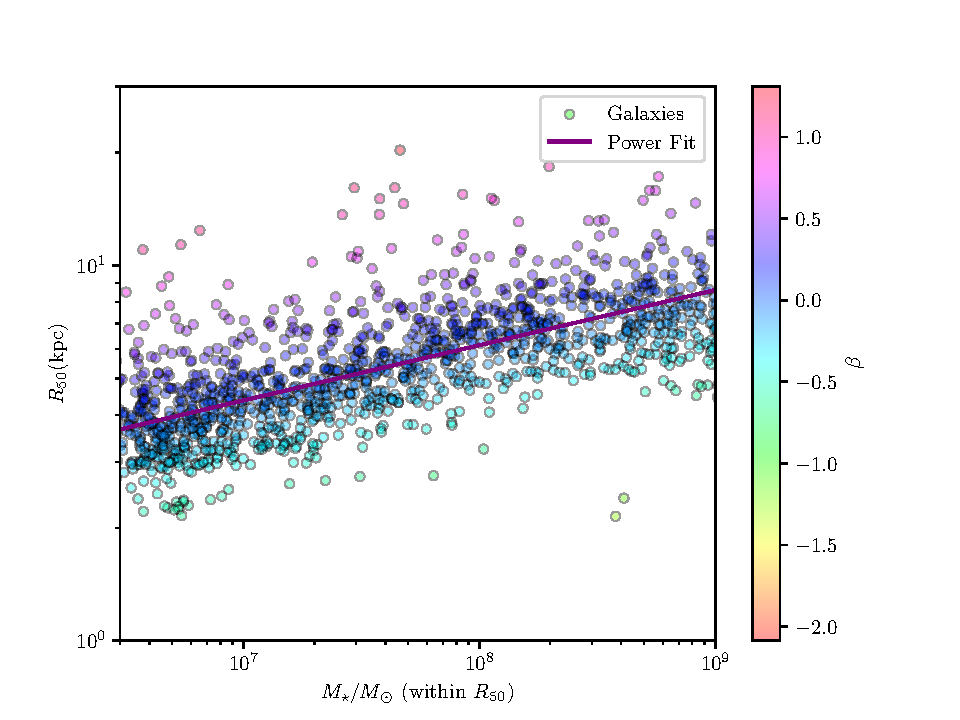
\includegraphics[width=\textwidth*2/3]{figs/me/stars-mass-size-r50.pdf}
    \caption{
        The left shows the size-mass relationship for the FIREbox low-mass galaxies. It covers the range $3 \times 10^3$ -- $1 \times 10^9 M_\odot$. Galaxies larger than this are no longer dwarfs and do not follow the power law, and galaxies smaller than this approach FIREbox's resolution limit. The line of best fit is described by equation (\ref{equ:linear-rel}) and $\beta$ represents the deviation from that line. $\beta$ is chosen to characterize the diffuseness of a galaxy because the distribution of $\beta$ is independent of mass for low-mass galaxies (see Figure \ref{fig:beta-mass}).
    }
    \label{fig:size-mass}
\end{figure}

\section{The Diffuseness Parameter}
As diffuseness will be main subject of this paper, let us define it. The low-mass galaxies in FIREbox loosely follow a power law size-mass relationship (see Figure \ref{fig:size-mass}). The relationship can therefore be described using the following equation,
\begin{equation}
    \frac{R_{50}}{1 kpc} \approx a
    \left(
        \frac{M_\star}{M_\odot}
    \right)
    ^{\gamma}
\end{equation}
where $\gamma$ and $a$ are constants and $M_\odot$ is the mass of the sun. I am dividing by a kiloparsec unit to make the equation unitless. Taking the logarithm of this equation yields
\begin{equation}
    \label{equ:linear-rel}
    \ln \left(
        \frac{R_{50}}{1 \text{ kpc}}
    \right)
    \approx
    \ln(a)
    + \gamma \ln \left(
        \frac{M_\star}{M_\odot}
    \right)
\end{equation}

By taking the natural logarithm of a power law, I end up with an equation for a line. This linear relationship can be seen in Figure \ref{fig:size-mass}. Here, $ln(a)$ becomes the $y$-intercept of the line and $\gamma$ becomes the slope. I have kept denoting this equation as \emph{approximately} equal in order to emphasize that not every galaxy falls exactly into this relationship. However, one can replace that by introducing a galaxy-specific parameter $\beta$ that is defined to be the galaxy's deviation from this linear relationship:
\begin{equation}
    \label{equ:log-log-with-beta}
    \ln \left(
        \frac{R_{50}}{1 kpc}
    \right)
    =
    \ln(a)
    + \gamma \ln \left(
        \frac{M_\star}{M_\odot}
    \right)
    + \beta
\end{equation} 

\begin{equation}
    \label{equ:beta}
    \beta
    \equiv
    \ln \left(
        \frac{R_{50}}{1 kpc}
    \right)
    -
    \ln(a)
    - \gamma \ln \left(
        \frac{M_\star}{M_\odot}
    \right)
\end{equation} 

I will call $\beta$ the \textbf{diffuseness parameter}, because it tells us how diffuse a galaxy is relative to its fellow galaxies. Positive values of $\beta$ mean that the galaxy has a larger radius than other galaxies of the same mass, and negative values mean a smaller radius. $\beta$ is especially useful for characterizing the diffuseness because the distribution of $\beta$ remains consistent across all masses of low-mass galaxies (see Figure \ref{fig:size-mass}). Note that this does not apply to galaxies larger than $10^9 M_\odot$ (see Figure \ref{fig:beta-mass}).


$\gamma$ and $\ln(a)$ are calculated using equation (\ref{equ:linear-rel}) and fitting the dataset to a line. One can then use those values in equation (\ref{equ:beta}) to find each galaxy's value of $\beta$. One can also characterize the \textbf{diversity of the diffuseness} of galaxies using the the standard deviation $\sigma_\beta$ (the mean is zero by design). I will use these values to compare FIREbox with the galaxies of the Local Group.

\begin{figure}
    \centering
    \includegraphics*[width=\textwidth*2/3]{figs/me/beta-mass.pdf}
    \caption{...}
    \label{fig:beta-mass}
\end{figure}

\section{Proximity}


 Tidal disruption may provide an explanation for diffuseness. Tidal forces are caused by a gradient in the gravitational field, that causes objects to be stretched. I inspected FIREbox galaxies' tidal interactions with their neighbors. Specifically, I examined a galaxy's distance to its nearest neighbor, as well as a satellite galaxy's distance to its host galaxy. For the distance to the host galaxy, I examined both the absolute separation and virial separation. I define the absolute separation to be the distance in kpc to the host galaxy, and the virial separation to be that distance as a fraction of the host galaxy's virial radius. The virial radius of a galaxy is the radius within which particles will tend to be gravitationally bound. In other words, it is the effective radius of a galaxy's gravitational well.

 \cite{jacksonDarkmatterdeficientDwarfGalaxies2021} defines the "perturbation index" (PI), which characterizes the strength of the tidal effect on an object in a virial halo. The PI is proportional to the inverse of the virial separation cubed. This power relationship means that we can test for tidal disruption using the virial separation.

 \subsection{Minimum Proximity}

 To determine whether tidal interactions affect the diffuseness of galaxies, it may be better to consider the \emph{minimum} distance between a satellite and its host, as opposed to the current distance. The minimum distance is the point at which the tidal forces are strongest, and therefore could cause the most extreme effects. I will therefore also compare $\beta$ to $d_{\rm{min}}$, using both the absolute and virial separation. Note that such an analysis is only possible with simulation data because we can only view the real universe in its present state. This analysis will exclude satellites that have not reached the perihelion of their trajectory.

\subsection{Calculating distances}

Calculating the distance between two galaxies in FIREbox is not as trivial as it may seem. The simulation volume is defined as a cube that repeats itself \citep{feldmannFIREboxSimulatingGalaxies2022}. In other words, if you travel across one border of the universe, you appear on the opposite side. This geometry is adopted to avoid any strange boundary conditions---it would be unrealistic for there to by enormous walls in space, for example. However, it is also impossible to simulate an infinite universe. This "wrapping around" model allows for a middle ground.

In order to measure the $x$ component of the distance between two objects one must first determine whether they are across the $x$ border. If they are, then one find the sum of the distances to the border. Otherwise, one finds the difference of their positions like normal. The same logic is used to find the $y$ and $z$ components. Only then does one calculate magnitude of the distance. Refer to Appendix \ref{apx:distances} for code to do this calculation.


